\chapter{電気と磁気を一つの相対論的場として}

我々は、与えられた電磁場が荷電粒子をどのように動かすかを学んできた。問題の未完成な半分は場そのものである。すなわち、電場と磁場がどのように発展し、電荷と電流がどのようにそれらの源として働くかである。マクスウェル方程式がこれらの問いに答える。しかし、それを書き下す前に、その相対論的構造を不可避にした物理的パズルを思い出す価値がある。

これは形式主義からの意図的な後退である。作用原理は再び戻ってくるが、まだではない。別のところから始める要点は、電場と磁場が一つの対象の部分でなければならない理由を、その力学を作用から導出する前に見ることにある。

\section{アインシュタインの最初の段落にあるパズル}

ベルギーへの訪問中に、初期のソルベー会議についての議論が、アインシュタインの1905年の論文\emph{運動物体の電気力学について}へと戻った。その最初の段落は、動機を驚くほど簡潔に述べている。同じ電磁現象が、二つの慣性系で一見異なる二つの説明を受ける。一方の観測者はその効果を磁気的と呼び、他方は電気的と呼ぶ。観測される運動は一致するので、二つの記述は物理学の異なる二つの部分を表すことはできない。

この論文は今や、この講義で展開された水準で理解できる。すべての計算をたどらなくても、冒頭の段落は読む価値がある。なぜならそれは、答えを導入する前に正しい問いを立てているからである。物理的出来事が変わらないのに、電気的記述と磁気的記述はどのように変わりうるのか。

\subsection{電荷、磁石、そして二つの記述}

\(y\)方向を向く磁場と、\(x\)軸に沿って運動する電荷を考える。実験室系では電場が消えるので、力は磁気的である。
\begin{equation}
\mathbf F=q\,\mathbf v\times\mathbf B.
\end{equation}
それは残りの横方向を向く。講義の素早い黒板の座標軸は、右手の法則のすべての符号を固定するためのものではない。重要な事実は、力が\(\mathbf v\)と\(\mathbf B\)の両方に垂直であること、そして電荷の符号を逆にすると力が逆になることである。

\begin{classroomqa}
\audiencequestion{図では、力は上を向くか下を向くか。}
\lecturerresponse{それは電荷の符号に依存する。座標軸の向きと\(q\)の符号が固定されれば、右手の法則が方向を決める。現在の議論では、横方向の力が存在することだけが重要である。\lecturetimestamp{00:07:13}}
\end{classroomqa}

アインシュタインは孤立した粒子ではなく導線について述べた。原子はほぼ固定された格子を提供し、可動の電荷担体がその中を動く。二十世紀初頭には、導線中の電流は、一つの自由な荷電粒子の軌道よりもはるかに観測しやすかった。この区別はここでは本質的でない。磁場中の運動する担体は同じローレンツ力を受ける。

\begin{figure}[H]
\centering
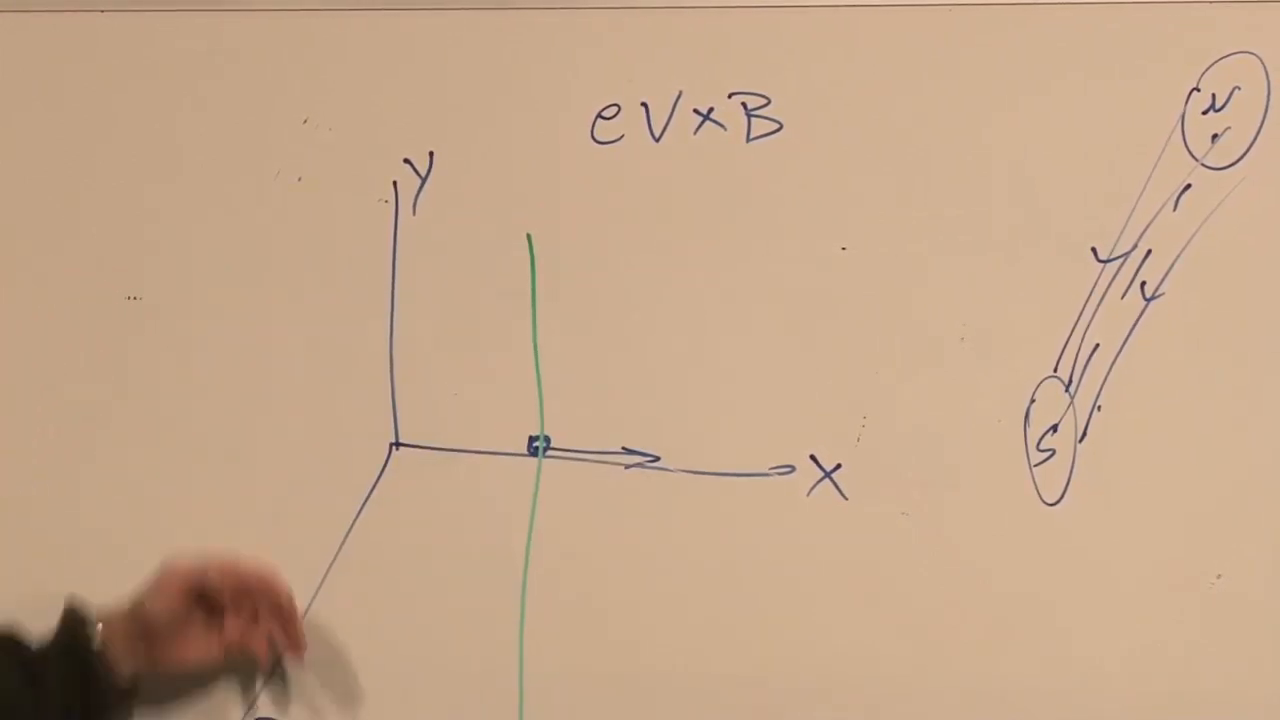
\includegraphics[width=\linewidth]{lecture_08_figure_01.png}
\caption{アインシュタインの電気力学のパズルを言い換えるために用いられる、運動する電荷、横方向の磁場、および磁石の幾何学的配置。}
\par\smallskip
\textit{講義のフレーム：00：07：00。}
\end{figure}

次に、導線、または試験電荷を固定し、代わりに磁石を動かす。変化する磁気配置は起電力を生み、それは局所的な言葉では電場である。その電場は静止した電荷を同じ横方向に押す。したがって二つの記述は
\begin{align}
\text{moving charge, fixed magnet:}\quad&
q\,\mathbf v\times\mathbf B,
\\
\text{fixed charge, moving magnet:}\quad&
q\,\mathbf E'.
\end{align}
相対運動は同じである。それゆえ相対性理論は、一方の系で純粋に磁気的である場が、別の系で電気的成分を獲得する仕組みを説明しなければならない。

電気と磁気は別個の実体ではない。それらは一つの相対論的場の、系に依存する部分である。アインシュタインはまだ現代的な場のテンソル記法を持っておらず、この段落で必要な系の変化をローレンツ変換とは呼んでいなかった。それにもかかわらず、変換の問題はすでに完全に存在している。

\section{電磁場テンソル}

電気的データと磁気的データを一緒に運ぶことができる対象は、反対称テンソル
\begin{equation}
F_{\mu\nu}
=
\partial_\mu A_\nu-\partial_\nu A_\mu.
\label{eq:field-tensor-definition}
\end{equation}
である。ギリシャ文字の添字は\(0,1,2,3\)を走り、\(x^0=t\)である。ラテン文字の添字は三つの空間値を走る。反対称性
\begin{equation}
F_{\mu\nu}=-F_{\nu\mu},
\end{equation}
は対角成分をゼロにし、六つの独立な成分を残す。それら六つはまさに\(\mathbf E\)の三つの成分と\(\mathbf B\)の三つの成分である。

mostly-plus の計量
\begin{equation}
\eta_{\mu\nu}=\operatorname{diag}(-1,1,1,1),
\end{equation}
と、前回の講義の荷電粒子の作用から受け継いだ規約のもとで、
\begin{align}
E_m&=F_{0m}
=\partial_0A_m-\partial_mA_0,
\label{eq:e-from-a}
\\
B_i&=(\boldsymbol\nabla\times\mathbf A)_i.
\label{eq:b-from-a}
\end{align}
と定義する。講義では最初の行を書く際に空間添字を訂正している。正しい関係は上記のものである。すなわち、自由な空間添字は両辺で一致しなければならない。

\begin{figure}[H]
\centering
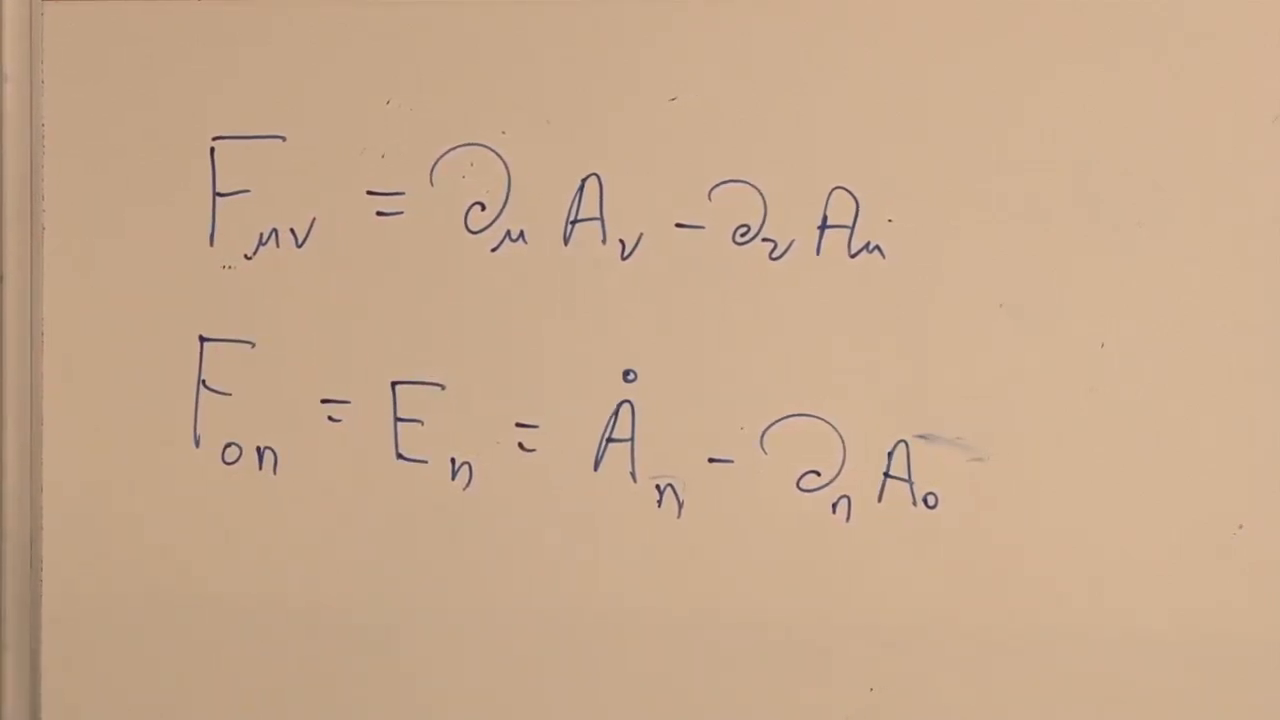
\includegraphics[width=\linewidth]{lecture_08_figure_02.png}
\caption{場のテンソルの定義と、電場と同一視される混合時間--空間成分。}
\par\smallskip
\textit{講義のフレーム：00:13:15。}
\end{figure}

磁場の関係は同じ定義の空間部分である。例えば、
\begin{equation}
B_x
=
\partial_yA_z-\partial_zA_y
=
F_{yz},
\end{equation}
であり、他の二つの成分は巡回置換によって得られる。

\begin{figure}[H]
\centering
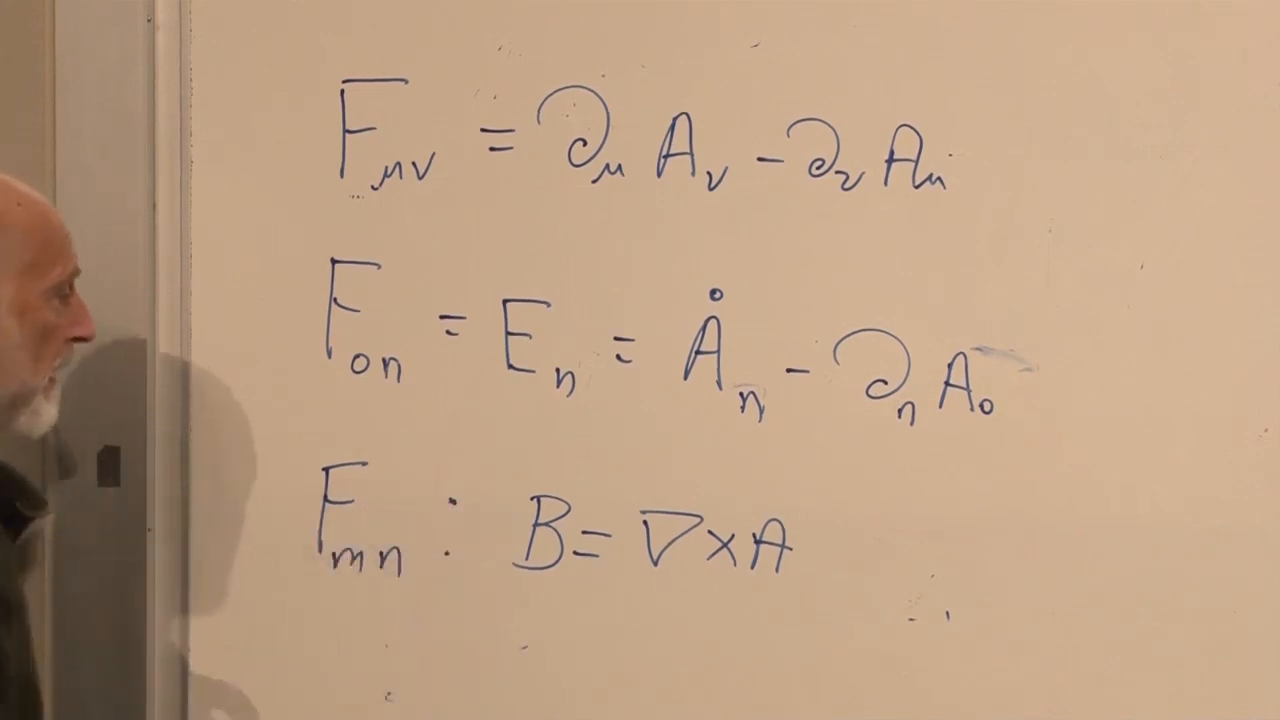
\includegraphics[width=\linewidth]{lecture_08_figure_03.png}
\caption{電場と磁場の回転に対するベクトルポテンシャルの公式を板書でまとめたもの。}
\par\smallskip
\textit{講義のフレーム：00:14:00。}
\end{figure}

\subsection{成分の配列}

第一のテンソル添字が行を、第二の添字が列を表すとし、\(0,x,y,z\)の順に並べる。すると
\begin{equation}
F_{\mu\nu}
=
\begin{pmatrix}
0&E_x&E_y&E_z\\
-E_x&0&B_z&-B_y\\
-E_y&-B_z&0&B_x\\
-E_z&B_y&-B_x&0
\end{pmatrix}.
\label{eq:f-lower-matrix}
\end{equation}
混合時間--空間の辺には\(\mathbf E\)が入り、空間的な\(3\times3\)ブロックには\(\mathbf B\)が入る。下三角は新しい情報ではない。なぜなら、それは上三角の負の鏡映だからである。

\begin{figure}[H]
\centering
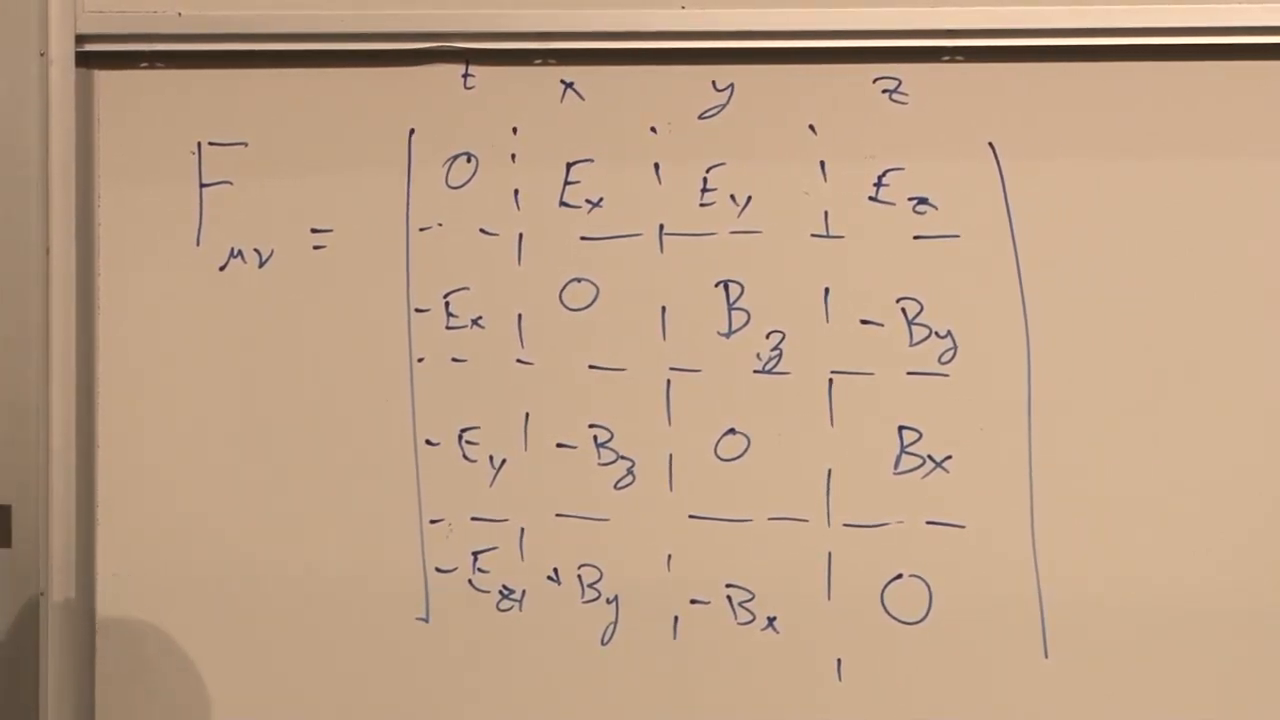
\includegraphics[width=\linewidth]{lecture_08_figure_04.png}
\caption{電場の辺と磁場の空間ブロックを備えた、完成した下添字の電磁テンソル。}
\par\smallskip
\textit{講義のフレーム：00:17:15。}
\end{figure}

両方の添字を上げると、すべての電場の成分の符号が変わり、磁場の成分は変わらない：
\begin{equation}
F^{\mu\nu}
=
\begin{pmatrix}
0&-E_x&-E_y&-E_z\\
E_x&0&B_z&-B_y\\
E_y&-B_z&0&B_x\\
E_z&B_y&-B_x&0
\end{pmatrix}.
\label{eq:f-upper-matrix}
\end{equation}
電場の成分は時間添字を一つ持つので、マイナス符号を一つ受け取る。磁場の成分は空間添字を二つ持つので、マイナス符号を受け取らない。

\begin{classroomqa}
\audiencequestion{磁場の成分には時間添字がないと、この行列を読んで理解してよいのでしょうか。}
\lecturerresponse{はい。それらは純粋に空間的なブロックを占めています。電場の成分はまさに、第一行と第一列に沿った混合時間--空間の成分です。\lecturetimestamp{00:18:55}}
\end{classroomqa}

\section{純粋な磁場をブーストする}

\(x\)に沿ったブーストを考え、\(c=1\)とする：
\begin{align}
t'&=\gamma(t-vx),
&
x'&=\gamma(x-vt),
&
y'&=y,
&
z'&=z,
\end{align}
ここで
\begin{equation}
\gamma=\frac{1}{\sqrt{1-v^2}}.
\end{equation}
行列の形では、
\begin{equation}
x'^\mu
=
\Lambda^\mu{}_\nu x^\nu,
\qquad
\Lambda^\mu{}_\nu
=
\begin{pmatrix}
\gamma&-\gamma v&0&0\\
-\gamma v&\gamma&0&0\\
0&0&1&0\\
0&0&0&1
\end{pmatrix}.
\label{eq:x-boost}
\end{equation}

\begin{classroomqa}
\audiencequestion{ブースト行列にマイナス符号が一つ欠けていませんか。}
\lecturerresponse{はい。非対角の時間--空間成分は、\(t'=\gamma(t-vx)\)と
\(x'=\gamma(x-vt)\)によって要求されるマイナス符号を持っています。この修正は、場の変換を用いる前に行われます。\lecturetimestamp{00:23:50}}
\end{classroomqa}

\begin{figure}[H]
\centering
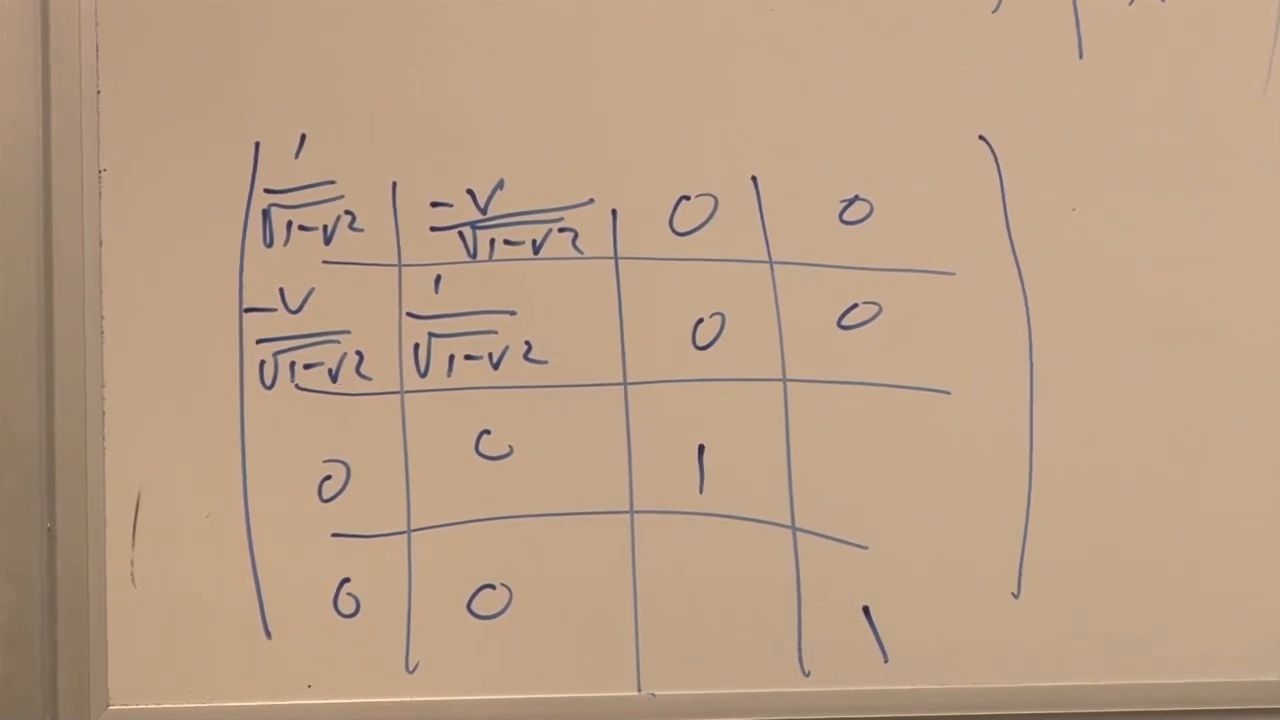
\includegraphics[width=\linewidth]{lecture_08_figure_05.png}
\caption{\(x\)軸に沿った運動に対する、修正されたローレンツ・ブースト行列。}
\par\smallskip
\textit{講義のフレーム：00:24:00。}
\end{figure}

すべての上付きテンソル添字は、上付きベクトル添字と同じように変換される。したがって
\begin{equation}
F'^{\mu\nu}
=
\Lambda^\mu{}_\sigma
\Lambda^\nu{}_\tau
F^{\sigma\tau}.
\label{eq:f-boost-law}
\end{equation}
繰り返されている\(\sigma\)と\(\tau\)はダミー添字である。より多くの添字を持つテンソルでは、各添字に対して変換行列が一つ現れることになる。

\begin{figure}[H]
\centering
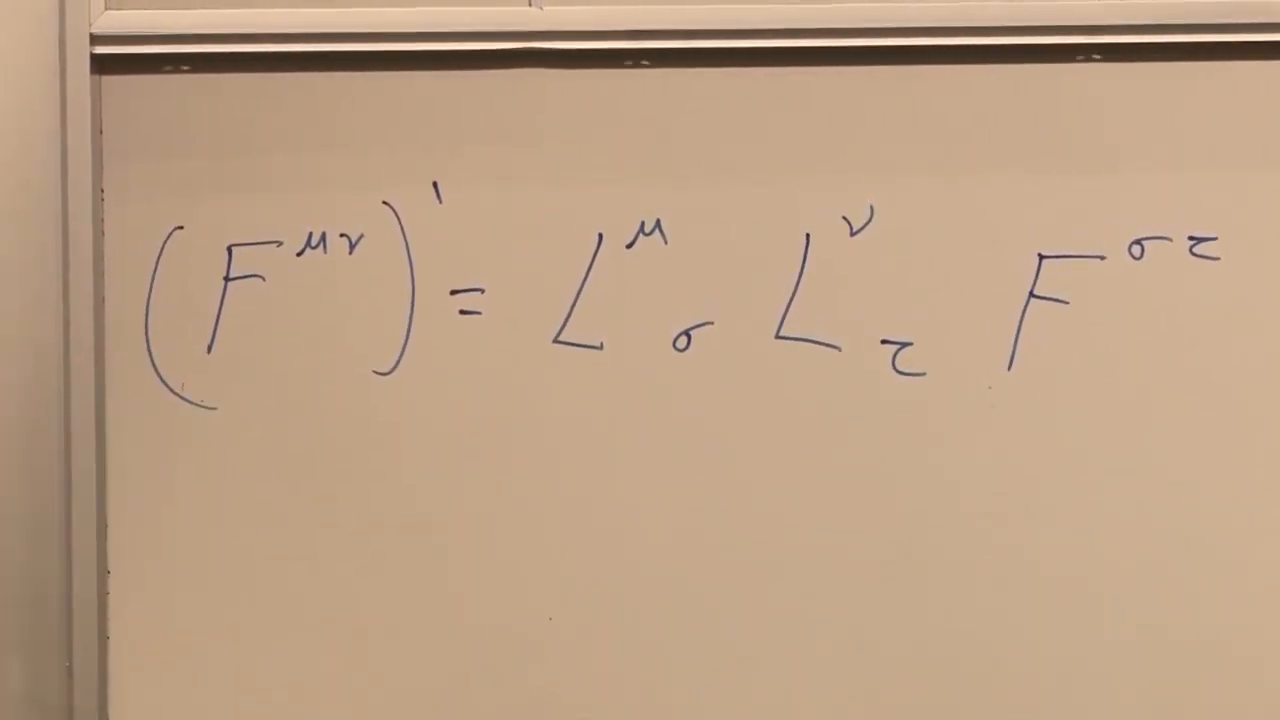
\includegraphics[width=\linewidth]{lecture_08_figure_06.png}
\caption{階数二のローレンツ変換則であり、場のテンソルの各添字に対してブースト行列が一つある。}
\par\smallskip
\textit{講義のフレーム：00:26:40。}
\end{figure}

\subsection{電場になる成分}

プライムの付いていないフレームには磁場\(B_y\)だけが含まれると仮定する。式~\eqref{eq:f-upper-matrix}の規約では、関連する独立な成分は
\begin{equation}
F^{xz}=-B_y.
\end{equation}
である。我々はプライムの付いた混合成分\(F'^{0z}\)を求める。なぜなら、それは電場のプライムの付いた\(z\)成分を担うからである。式
\eqref{eq:f-boost-law}より
\begin{align}
F'^{0z}
&=
\Lambda^0{}_\sigma
\Lambda^z{}_\tau F^{\sigma\tau}
\\
&=
\Lambda^0{}_x\Lambda^z{}_zF^{xz}
\\
&=
(-\gamma v)(1)(-B_y)
=
\gamma vB_y.
\end{align}
この規約では\(F'^{0z}=-E'_z\)であるから、
\begin{equation}
E'_z=-\gamma vB_y.
\label{eq:boosted-electric-field}
\end{equation}
符号は宣言された軸と場の規約に依存する。計算の不変な要点は
\begin{equation}
\lvert E'_z\rvert
=
\gamma\lvert vB_y\rvert
\ne0.
\end{equation}
である。二重和は、元の場がこの一つの独立な磁場の成分しか持たないために潰れる。

\begin{figure}[H]
\centering
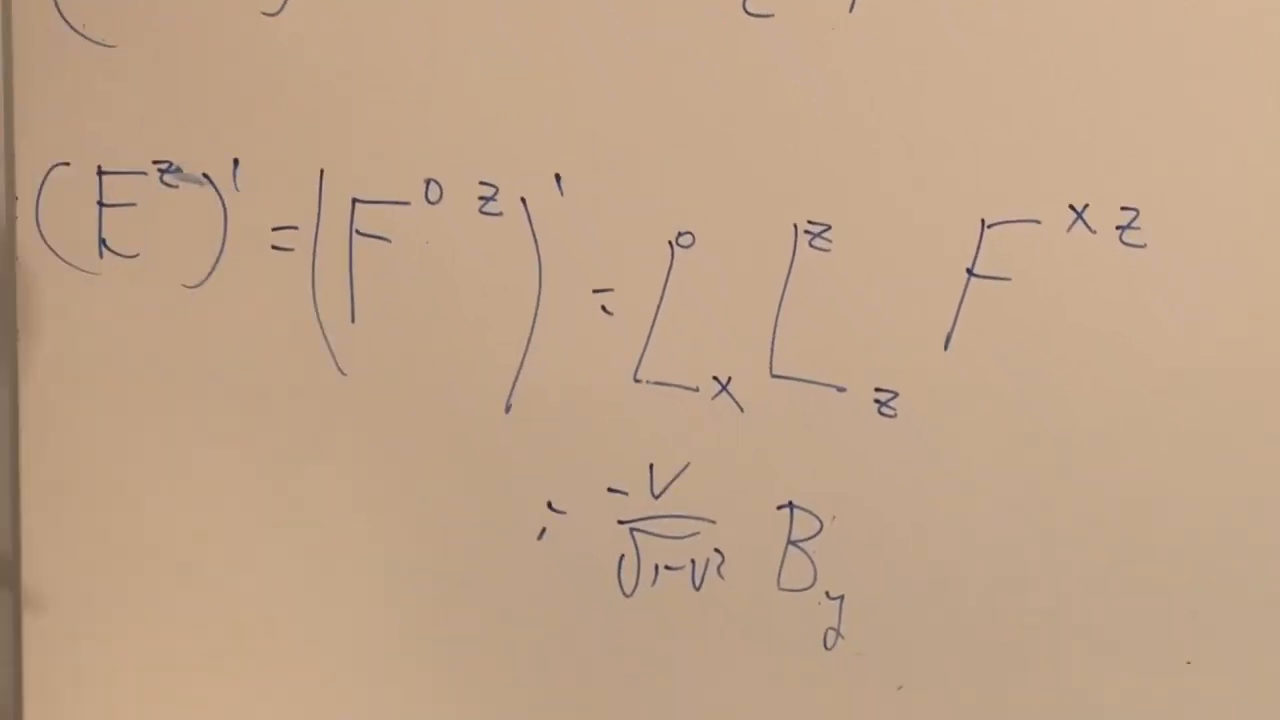
\includegraphics[width=\linewidth]{lecture_08_figure_07.png}
\caption{ブースト後の選択されたテンソル成分であり、元の磁場の成分に掛かる因子\(\gamma v\)を示している。}
\par\smallskip
\textit{講義のフレーム：00:32:30。}
\end{figure}

プライムの付いたフレームが電荷とともに動くように選ぶ。すると電荷は静止しているので、その力の磁場の部分\(q\,\mathbf v'\times\mathbf B'\)はない。それでも力は消えない。それは\(q\mathbf E'\)である。実験室の観測者にとっての磁場の力と、共動する観測者にとっての電場の力は、同じ事象の二つの記述である。

これがアインシュタインの最初の段落にあるパズルへの答えである。この問いはこの講義のおよそ最初の四十分を占めた。歴史的な冗談は、それがアインシュタインをはるかに長く占めたということである。この計算に時間を費やす価値があるのは、電場と磁場が混ざるというスローガンを、一つの明示的なテンソル成分に変えてくれるからである。

\section{マクスウェル方程式：恒等式と力学}

ここで、電荷に働く力から場の方程式へと移る。それらは次の講義で作用から導かれる。ここでの目的は、まずそれらを述べ、その二つの異なる論理的な役割を理解し、恒等式に基づく半分を共変形式に置くことである。

\begin{classroomqa}
\audiencequestion{これらの方程式はすでに導出したのではないか。}
\lecturerresponse{我々が導出したのは、与えられた電磁場中における荷電粒子の運動方程式である。マクスウェル方程式は場そのものの運動方程式であり、電荷および電流に対する場の応答を含んでいる。\lecturetimestamp{00:35:10}}
\end{classroomqa}

\begin{classroomqa}
\audiencequestion{マクスウェル方程式はいくつあるのか。}
\lecturerresponse{スカラー成分方程式は8本ある。ベクトル記法では、それらは2本のスカラー方程式と2本の3成分ベクトル方程式にまとめられ、慣例的に4本のマクスウェル方程式と呼ばれる。\lecturetimestamp{00:35:24}}
\end{classroomqa}

\(c=1\) とし、通常の真空定数を電荷と電流の定義に吸収した単位系を引き続き用いる。8本の成分方程式のうち4本は定義 \(F=dA\) から従う。それらは運動学的な恒等式である。残りの4本は動的であり、場の作用が変われば変化しうる。

\subsection{3つの基本的なベクトル演算}

微分可能な3次元ベクトル場 \(\mathbf A\) に対して、
\begin{align}
(\boldsymbol\nabla\times\mathbf A)_x
&=
\partial_yA_z-\partial_zA_y,
\\
\boldsymbol\nabla\cdot\mathbf A
&=
\partial_xA_x+\partial_yA_y+\partial_zA_z.
\end{align}
残りの回転の成分は \(x\to y\to z\to x\) を巡回置換することで得られる。スカラー場 \(s\) に対して、
\begin{equation}
\boldsymbol\nabla s
=
(\partial_xs,\partial_ys,\partial_zs).
\end{equation}
したがって、回転はベクトルであり、発散はスカラーであり、勾配はベクトルである。

\begin{classroomqa}
\audiencequestion{回転と発散の定義を完全に復習する必要がある人はいるか。}
\lecturerresponse{成分による定義は記録されているが、残りの成分をすべて展開する必要はない。座標ラベルを巡回させることでそれらが得られる。\lecturetimestamp{00:37:32}}
\end{classroomqa}

滑らかな偏微分の可換性は2つの恒等式を意味する。
\begin{align}
\boldsymbol\nabla\cdot
(\boldsymbol\nabla\times\mathbf A)
&=0,
\label{eq:div-curl}
\\
\boldsymbol\nabla\times
(\boldsymbol\nabla s)
&=\mathbf0.
\label{eq:curl-grad}
\end{align}

\begin{classroomqa}
\audiencequestion{回転の発散がゼロになることの完全な成分による証明を書き出すべきか。}
\lecturerresponse{クラスは辞退する。成分を展開すると \(\partial_x\partial_yA_z\) や
\(-\partial_y\partial_xA_z\) のような対が生じ、微分の順序を入れ替えられるため相殺する。\lecturetimestamp{00:40:13}}
\end{classroomqa}

\begin{figure}[H]
\centering
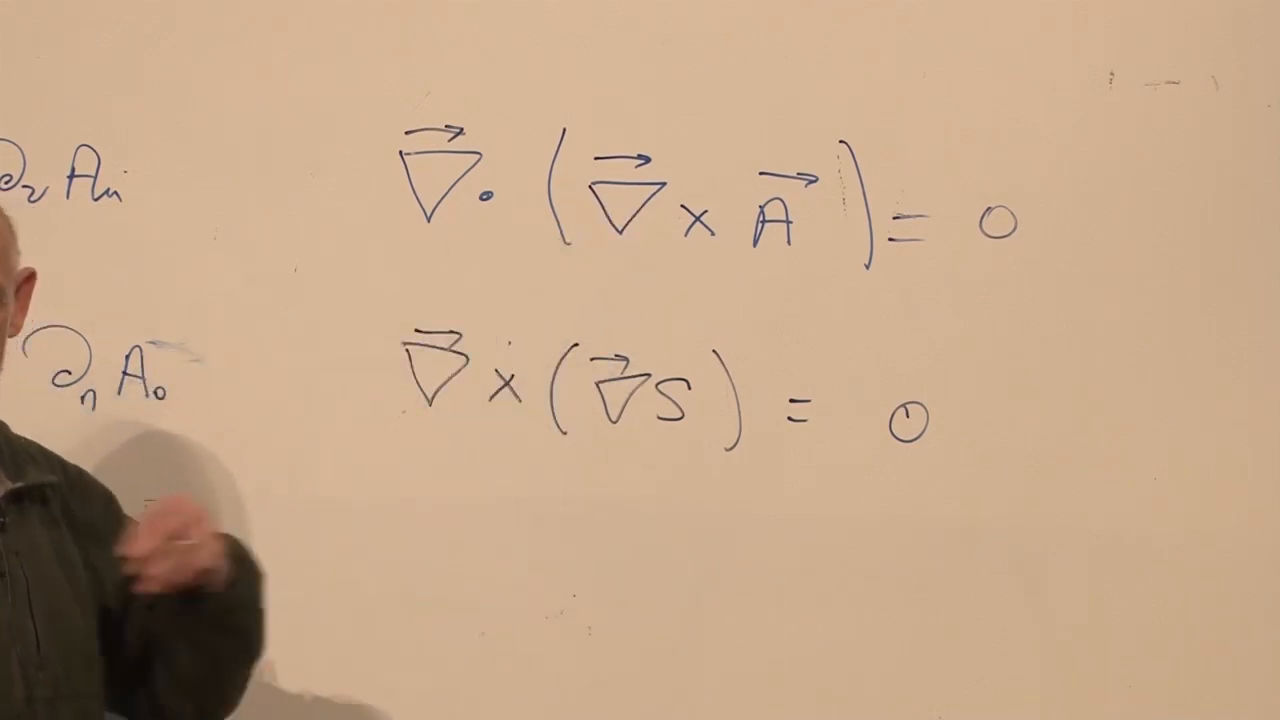
\includegraphics[width=\linewidth]{lecture_08_figure_08.png}
\caption{マクスウェル方程式の半分を得るために用いられた、回転の発散および勾配の回転の恒等式。}
\par\smallskip
\textit{講義フレーム: 00:41:40.}
\end{figure}

\subsection{ベクトルポテンシャルから磁場の源は生じない}

式~\eqref{eq:b-from-a}の発散を取ると
\begin{equation}
\boldsymbol\nabla\cdot\mathbf B
=
\boldsymbol\nabla\cdot
(\boldsymbol\nabla\times\mathbf A)
=0.
\label{eq:div-b-zero}
\end{equation}
運動方程式は用いていない。この結果はポテンシャルによる記述と滑らかな微分のみから従う。

\begin{figure}[H]
\centering
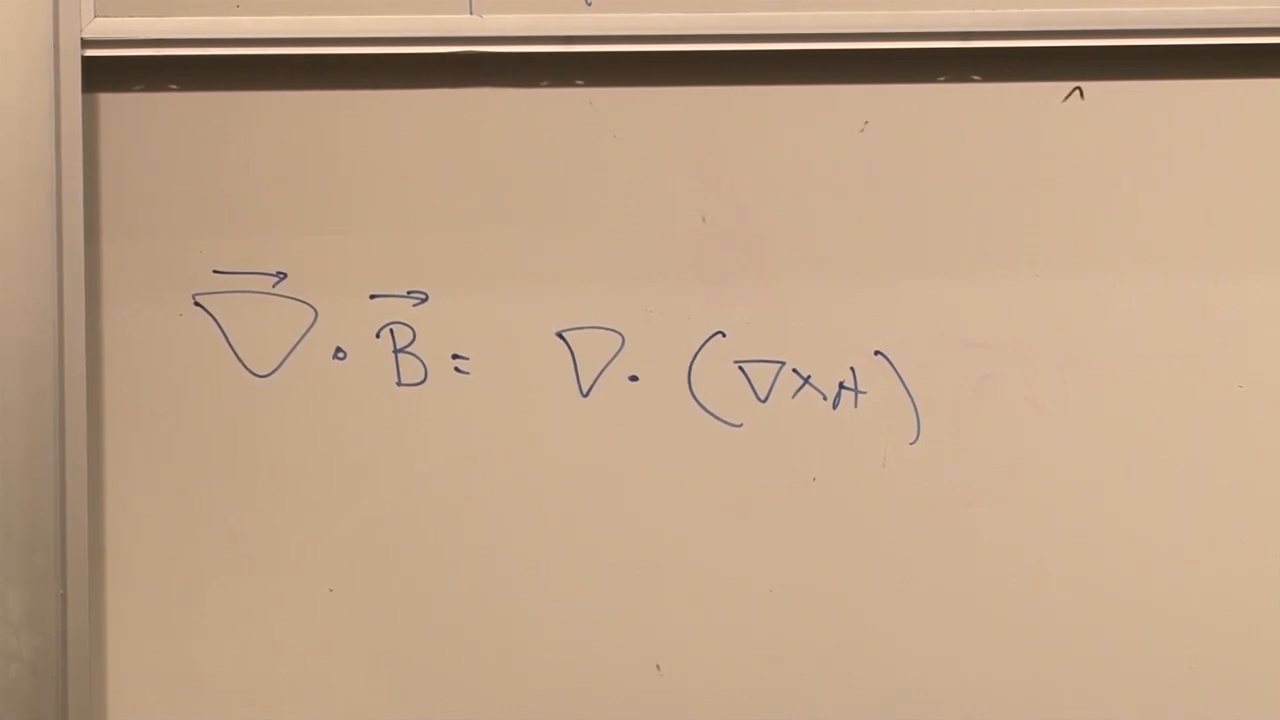
\includegraphics[width=\linewidth]{lecture_08_figure_09.png}
\caption{磁場の発散は回転の発散に帰着した。}
\par\smallskip
\textit{講義フレーム: 00:43:05.}
\end{figure}

\begin{classroomqa}
\audiencequestion{電場の発散は何か。}
\lecturerresponse{それは用いている単位系における電荷密度 \(\boldsymbol\nabla\cdot\mathbf E=\rho\) である。点電荷は、源から広がる電場の電気力線の原型である。
\lecturetimestamp{00:43:20}}
\end{classroomqa}

この初等的な段階では、式~\eqref{eq:div-b-zero}は磁荷密度が存在しないことを述べている。滑らかで大域的に定義されたベクトルポテンシャルは磁気単極子の源を生み出せない。後にこの主張は限定されなければならない。単極子は、重なり合うパッチ上で定義されたポテンシャルや特異なゲージ選択によって記述できる。講義ではその精密化を後回しにする。

\subsection{電位からのファラデーの方程式}

式~\eqref{eq:e-from-a}は、3次元ベクトル記法では
\begin{equation}
\mathbf E
=
\frac{\partial\mathbf A}{\partial t}
-\boldsymbol\nabla A_0.
\label{eq:e-vector-potential}
\end{equation}
\(A_0\) は4元ベクトルに属するが、通常の空間回転の下ではスカラーである。回転を取ると:
\begin{align}
\boldsymbol\nabla\times\mathbf E
&=
\boldsymbol\nabla\times
\frac{\partial\mathbf A}{\partial t}
-
\boldsymbol\nabla\times
(\boldsymbol\nabla A_0)
\\
&=
\frac{\partial}{\partial t}
(\boldsymbol\nabla\times\mathbf A)
\\
&=
\frac{\partial\mathbf B}{\partial t}.
\end{align}
空間的回転は時間微分と可換であり、勾配の回転はゼロである。

\begin{figure}[H]
\centering
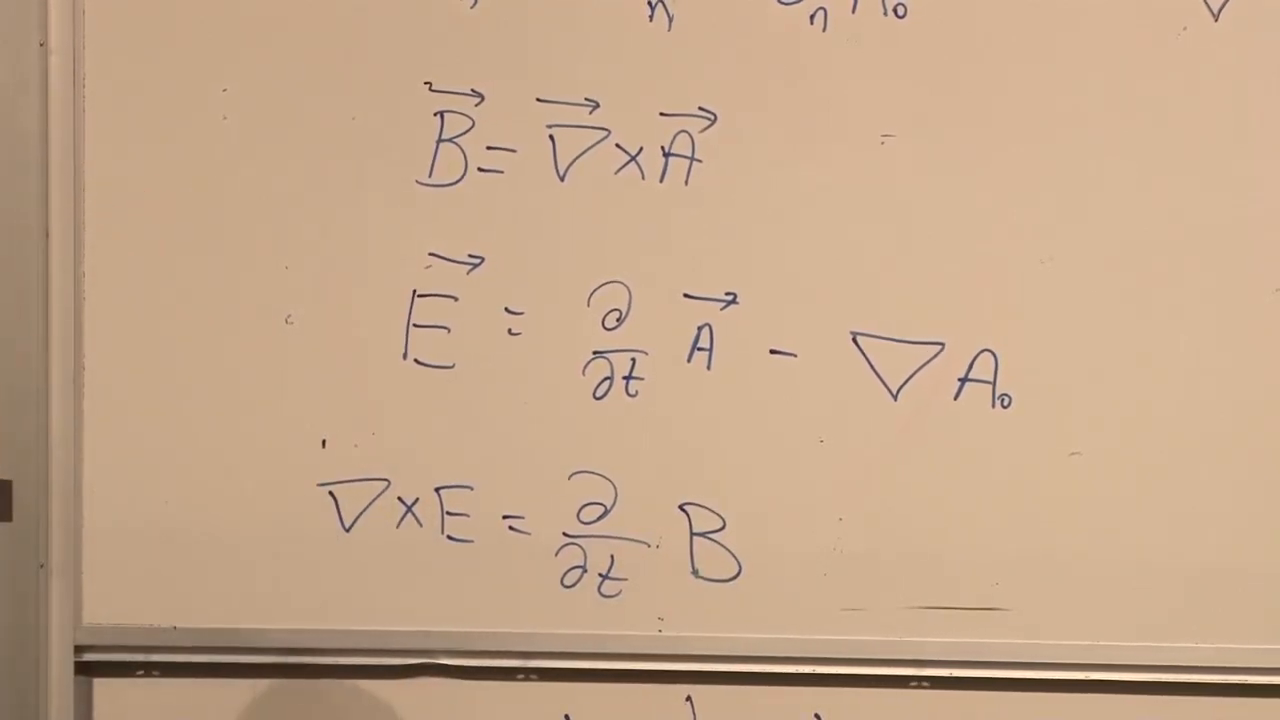
\includegraphics[width=\linewidth]{lecture_08_figure_10.png}
\caption{磁場の回転、電位の公式、および回転の計算の冒頭を1つの完成した板書状態にまとめたもの。}
\par\smallskip
\textit{講義フレーム: 00:47:45.}
\end{figure}

したがって、4本の同次成分方程式は
\begin{align}
\boldsymbol\nabla\cdot\mathbf B&=0,
\label{eq:homogeneous-div}
\\
\boldsymbol\nabla\times\mathbf E
-\frac{\partial\mathbf B}{\partial t}
&=\mathbf0.
\label{eq:homogeneous-curl}
\end{align}
最初のものは1本のスカラー方程式であり、2番目のものは3成分ベクトル方程式である。

\begin{figure}[H]
\centering
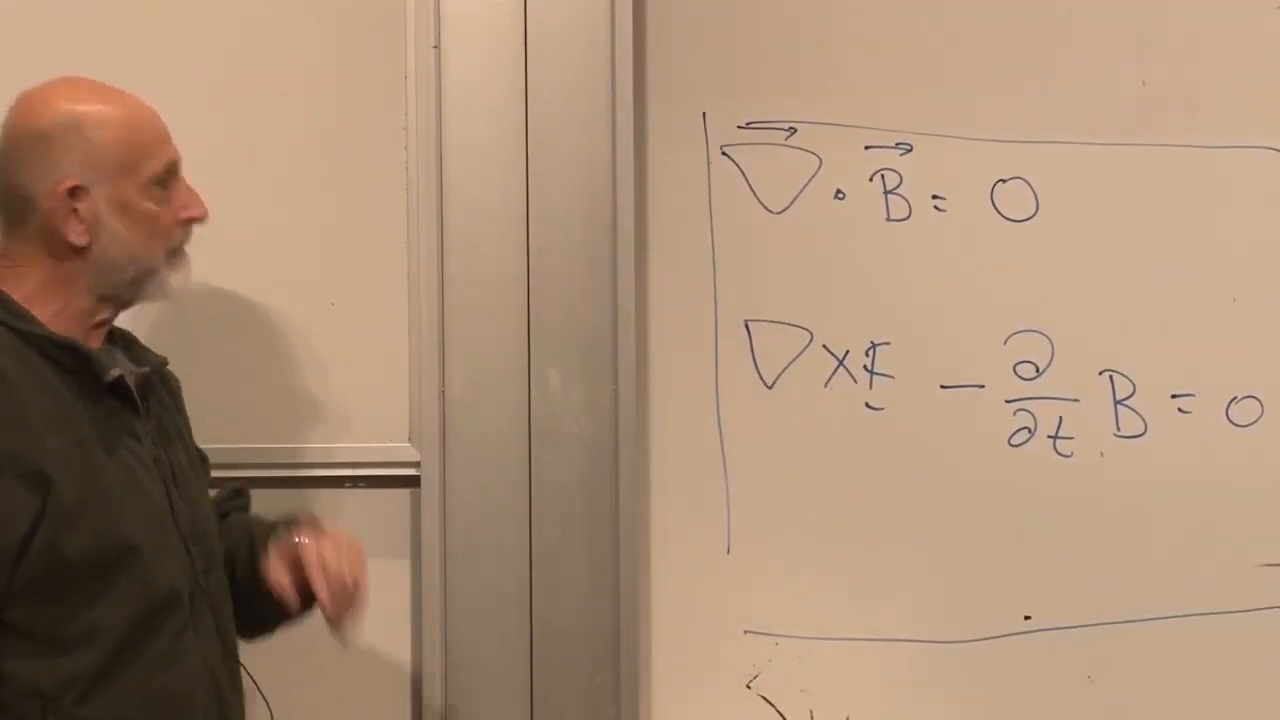
\includegraphics[width=\linewidth]{lecture_08_figure_11.png}
\caption{ポテンシャルの定義から直接得られる源のないマクスウェル方程式の対。}
\par\smallskip
\textit{講義フレーム: 00:48:45.}
\end{figure}

\subsection{動的な半分}

残りの方程式は
\begin{align}
\boldsymbol\nabla\cdot\mathbf E&=\rho,
\label{eq:gauss-electric}
\\
\boldsymbol\nabla\times\mathbf B
+\frac{\partial\mathbf E}{\partial t}
&=-\mathbf J.
\label{eq:ampere-maxwell}
\end{align}
これらは \(F=dA\) の帰結ではない。それらは源がどのように場を生成し変化させるかを記述しており、次の講義で電磁作用から導出する。電流の負符号はすでに選んだ規約によって固定されている: \(F_{0i}=E_i\)、
\(F_{ij}=\epsilon_{ijk}B_k\)、および
\(\partial_\mu F^{\mu\nu}=J^\nu\)。ライブ板書では当初、この負符号なしで \(\mathbf J\) が右辺に置かれる。その結果生じる電荷保存則との不一致は、次の講義で気づかれ修正される。

\begin{classroomqa}
\audiencequestion{回転の式の右辺にあるのはどのような量ですか。}
\lecturerresponse{左辺は3次元ベクトルであるから、右辺は電荷電流密度と呼ばれる3次元ベクトル\(\mathbf J\)である。ガウスの式の右辺は3次元スカラーである電荷密度\(\rho\)である。
\lecturetimestamp{00:50:36}}
\end{classroomqa}

\begin{figure}[H]
\centering
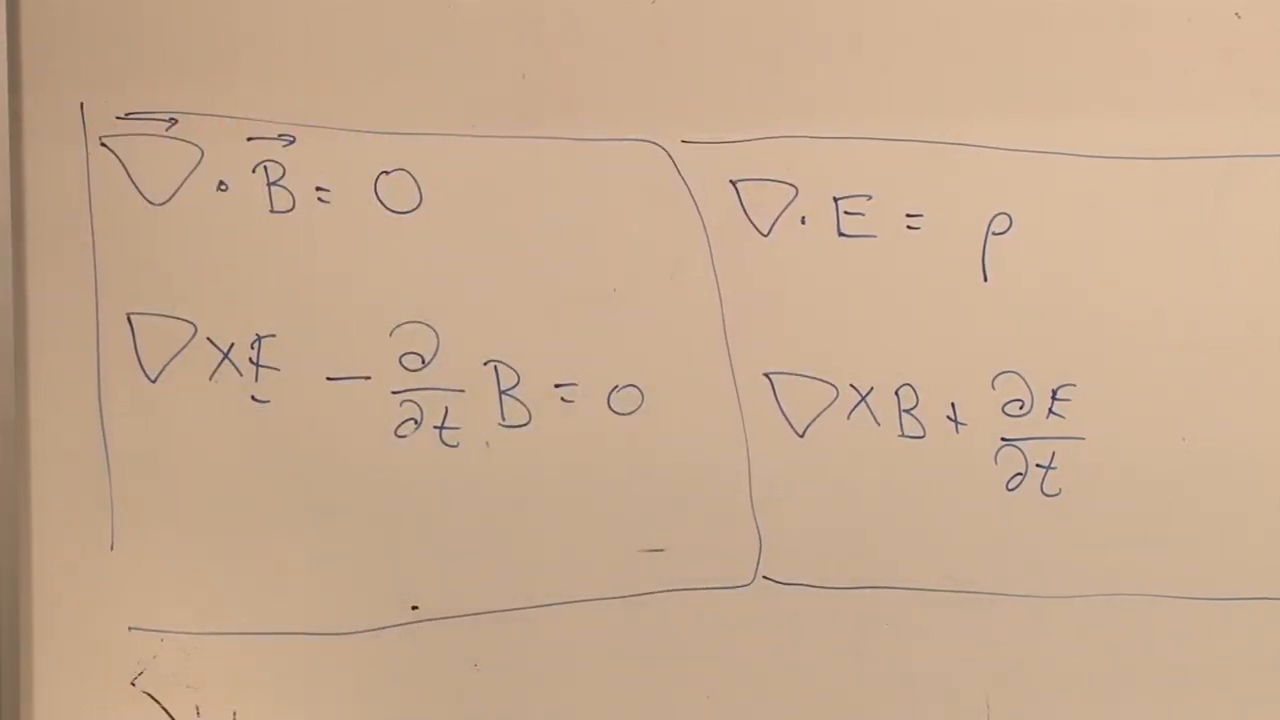
\includegraphics[width=\linewidth]{lecture_08_figure_12.png}
\caption{4つのマクスウェル方程式を、恒等式に基づく対と源をもつ動力学対にまとめたもの。}
\par\smallskip
\textit{講義フレーム: 00:50:40.}
\end{figure}

\section{時空の流れとしての電荷と電流}

記号\(\rho\)と\(\mathbf J\)には、ここで幾何学的な意味を与えなければならない。電荷密度は単位体積あたりの電荷であり、電流密度は単位時間あたりに有向面積を横切る電荷である。講義では、後にそれらが4元ベクトルとして統合されることが偶然に見えないように、両方を世界線から導く。

\subsection{隣の黒板からの教室余談}

それらの世界線を描く前に、隣室に見える方程式が短い教育的余談の機会となる。今後の講義では、量子場の理論と現代数学との関連に必要な背景を求める数学部の教員に量子力学を導入することになる。課題は双方向に及ぶ。物理学者は暗黙の物理的習慣を明示しなければならず、数学者は形式構造が何を記述するよう求められているのかを学ばなければならない。

\begin{classroomqa}
\audiencequestion{その教育任務が苛立たしいと感じるのは誰だと予想されますか。}
\lecturerresponse{おそらく双方である。すなわち、不慣れな聴衆を教える物理学者と、形式主義の背後にある物理的習慣に直面する数学者である。それでも、この任務は楽しいものになると予想される。その後、授業は電荷と電流に戻る。\lecturetimestamp{00:53:20}}
\end{classroomqa}

\subsection{電荷密度}

時間を縦に描き、残りの描かれた方向を3次元空間の代わりとする。荷電粒子は世界線を描く。ある固定された時刻において、体積\(\Delta V\)の小さな空間立方体をその世界線の束に重ね、その内部にある粒子の電荷を加える。電荷密度は
\begin{equation}
\rho(t,\mathbf x)
=
\lim_{\Delta V\to0}
\frac{\Delta Q}{\Delta V}.
\label{eq:charge-density}
\end{equation}
黒板上の2次元正方形は3次元立方体を表す。欠けている空間方向が省略されているのは、4次元を平らな黒板に描くことができないからにすぎない。

\begin{figure}[H]
\centering
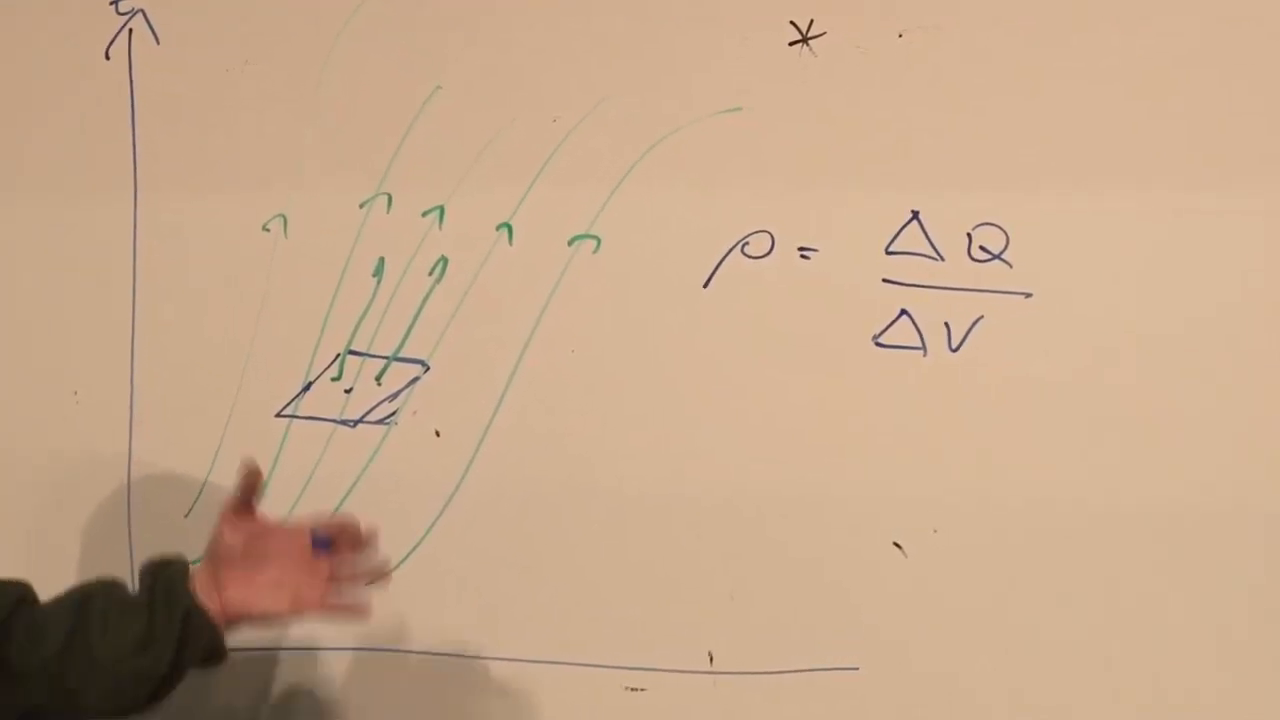
\includegraphics[width=\linewidth]{lecture_08_figure_13.png}
\caption{小さな空間セルを横切る荷電粒子の世界線。ただし\(\rho=\Delta Q/\Delta V\)。}
\par\smallskip
\textit{講義フレーム: 00:57:20.}
\end{figure}

\subsection{電流密度}

時空セルを横向きにする。\(J_x\)を定義するには、\(yz\)平面内に面積\(\Delta A_x\)の小さな窓を、\(x\)軸に垂直に選ぶ。\(\Delta t\)の間に負の\(x\)側から正の\(x\)側へ横切る正味の電荷を数える:
\begin{equation}
J_x
=
\lim_{\Delta A_x,\Delta t\to0}
\frac{\Delta Q_x}{\Delta A_x\,\Delta t}.
\label{eq:jx-window}
\end{equation}
向きが符号を与える。\(y\)と\(z\)に垂直な窓は、同様にして\(J_y\)と\(J_z\)を定義する。

黒板はその図と正直に格闘する。\(yz\)平面内の窓は、壁の窓というより天井の窓のように見える。単に、一度に表示できる以上の関連する軸が存在するのである。不変な定義は、スケッチがそうでなくても曖昧でない。

\begin{classroomqa}
\audiencequestion{図の中の窓は天井にありますか。}
\lecturerresponse{部屋の類推では、はい。重要なのは、その平面が\(x\)方向に垂直であることである。\(yz\)面積は、それを横切る\(x\)方向の電流を測る。\lecturetimestamp{00:59:38}}
\end{classroomqa}

\begin{figure}[H]
\centering
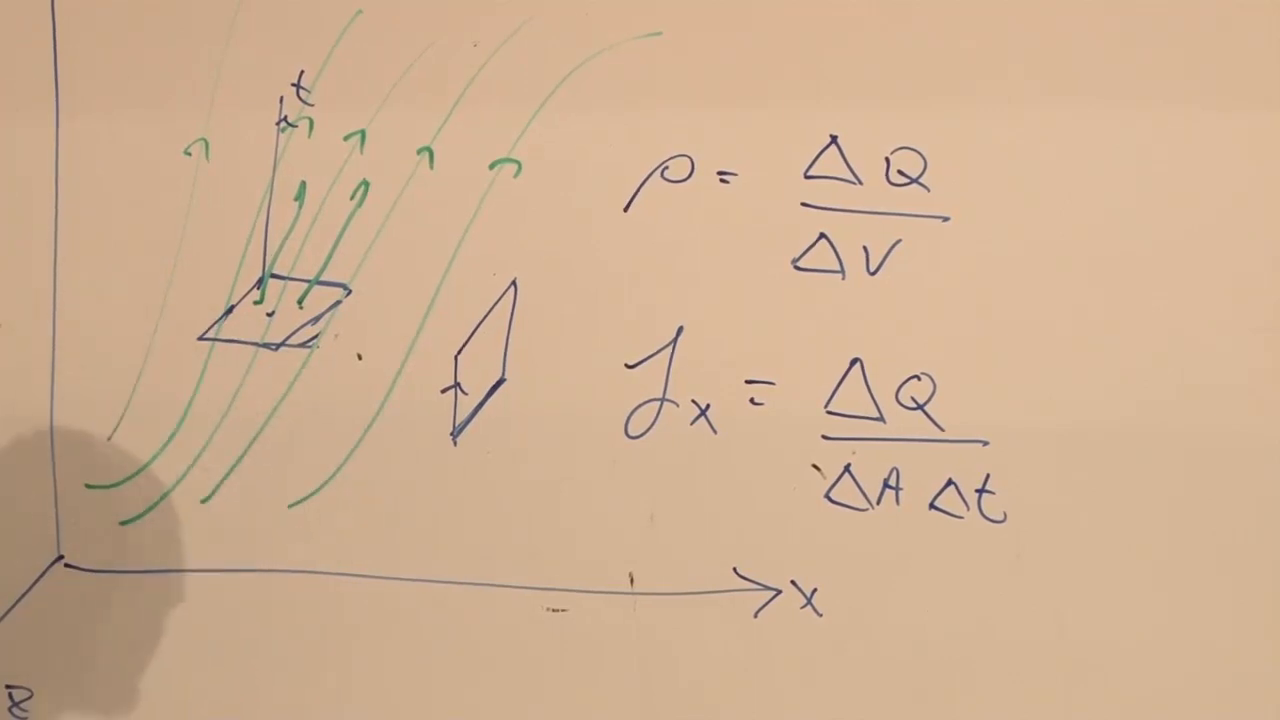
\includegraphics[width=\linewidth]{lecture_08_figure_14.png}
\caption{横断窓を通る電荷電流。ただし\(J_x=\Delta Q/(\Delta A\,\Delta t)\)。}
\par\smallskip
\textit{講義フレーム: 01:01:40.}
\end{figure}

\begin{figure}[H]
\centering
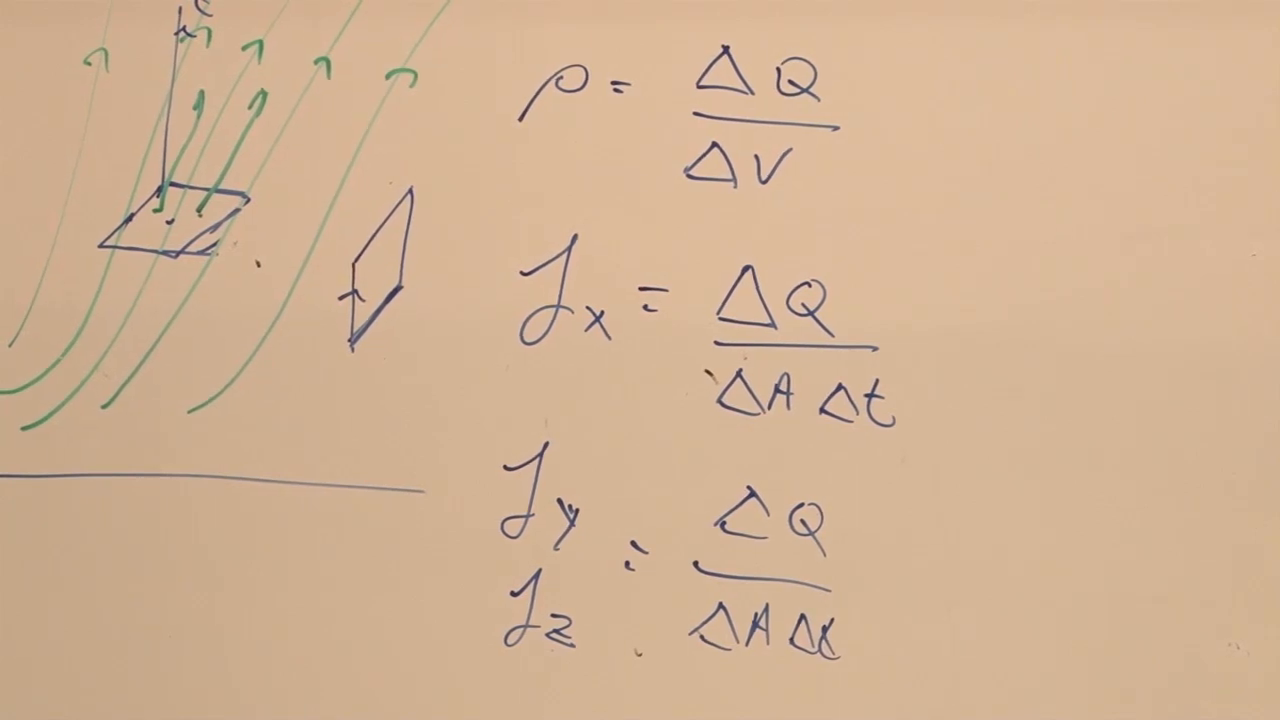
\includegraphics[width=\linewidth]{lecture_08_figure_15.png}
\caption{3つの空間軸に垂直な窓を横切る電荷によって定義される3つの電流成分。}
\par\smallskip
\textit{講義フレーム: 01:02:40.}
\end{figure}

4つの量は平行な定義をもつ。ある瞬間の空間体積は時間軸に垂直な超曲面であるから、\(\rho\)は時間に垂直な窓を通る電荷の流れである。\(J_i\)は空間に垂直な窓を通る流れである。

\begin{classroomqa}
\audiencequestion{4つの数は、時間方向の1つの流れと空間方向の3つの流れですか。}
\lecturerresponse{まさにそれが有用な描像である。空間体積は時間軸に垂直な窓であり、3つの横断面積は\(x\)、\(y\)、\(z\)に垂直な窓である。それらの4つの流束は一緒に属する。\lecturetimestamp{01:04:14}}
\end{classroomqa}

これは反変4元電流
\begin{equation}
J^\mu
=
(\rho,J_x,J_y,J_z).
\label{eq:four-current}
\end{equation}を示唆する

\begin{classroomqa}
\audiencequestion{計量はどこで入り、この電流は共変か反変か。}
\lecturerresponse{ここでの定義では、\(\rho\) と三つの \(J_i\) が \(J^\mu\) の成分をなし、これは上付き添字すなわち反変四元ベクトルである。\(J_\mu\) が必要なときには計量がその添字を下げる。上付き添字を選ぶのが自然である理由は、共変形式のマクスウェル方程式で示される。
\lecturetimestamp{01:04:48}}
\end{classroomqa}

\section{休憩時間の幕間：ブラックホール近傍の信号}

予定された休憩に入ると、質問は以前のブラックホールの議論に向けられた。これは電気力学からの脱線ではあるが、実質的な教室でのやり取りであり、異なる観測者による記述を区別するという同じ規律を示している。

\begin{classroomqa}
\audiencequestion{遠方の観測者が、落下する物体が事象の地平面近くで減速するのを見るなら、ブラックホールはこれまでにそこへ落ちたすべてのものに覆われて見えるべきだろうか。}
\lecturerresponse{シュヴァルツシルト座標時間では、古典的な落下は地平面に漸近的に近づくように見える。連続する物質は地平面近くでますます圧縮された層として思い描くことができる。しかし操作上は、外向きの信号はますます遅延し、赤方偏移し、微弱になる。通常の局所的な振動数で放出された光は、まず可視光として届き、次に赤外線、マイクロ波、電波として届き、各光子はより少ないエネルギーを運ぶ。現実的な遠方の検出器が明るく凍結した物体を永遠に見続けることはない。それは暗黒へと消えていく。
\lecturetimestamp{01:06:11}}
\end{classroomqa}

落下する観測者の時計と局所的に放出される懐中電灯は、その観測者にとって通常のままである。遠方からの記述が異なるのは、振動数と到着率が赤方偏移するからである。有限のエネルギーと有限の帯域幅のもとでは、実効的にメッセージの最後に分解可能な部分が存在する。

\begin{classroomqa}
\audiencequestion{その物体は事象の地平面に漸近的に近づいているのか。}
\lecturerresponse{それが遠方のシュヴァルツシルト座標による記述である。量子力学的には、消えていく信号はブラックホールのホーキング放射とも区別されなければならない。十分に遅い時刻には、弱く赤方偏移した信号は、ホール自身の放射の背景の中に観測上失われる。\lecturetimestamp{01:09:24}}
\end{classroomqa}

\begin{classroomqa}
\audiencequestion{赤方偏移した波長が観測可能な宇宙の尺度を超えて大きくなったらどうなるのか。}
\lecturerresponse{信号はその限界よりずっと早く、実際上失われる。講義では、光が一往復する時間あたりおよそ一つの典型的量子という、桁で見たホーキングの描像が与えられる。
\[
t_{\rm cross}\sim\frac{R_s}{c}.
\]
大きなホールにとってこれは極めて弱い放射であり、十分に赤方偏移した落下信号は、いかなる宇宙論的波長限界よりもずっと早く検出不能になる。\lecturetimestamp{01:09:50}}
\end{classroomqa}

\begin{classroomqa}
\audiencequestion{一往復時間あたりおよそ一つの量子という割合は、ブラックホールの生涯を通じて一定に保たれるのか。}
\lecturerresponse{いいえ。蒸発するシュヴァルツシルトブラックホールは縮小するので、その一往復時間は減少し、ホーキング温度は上昇する。したがって放出は加速する。瞬間的な半径による次元解析的な見積もりは依然として有用であるが、半径は一定ではない。対応して、典型的なホーキング波長は蒸発が進むにつれて短くなる。\lecturetimestamp{01:11:42}}
\end{classroomqa}

休憩の後、上着を脱いで、我々は \(\rho\) と \(\mathbf J\) に戻る。

\section{電荷の局所保存}

電荷保存を単に
\begin{equation}
\frac{dQ_{\rm universe}}{dt}=0.
\end{equation}
と述べるだけでは誘惑に駆られる。その主張は弱すぎる。電荷は実験室から消え、ケンタウルス座{\proseunicodefont α}星に、あるいはさらに遠くかみのけ座銀河団に瞬時に再出現しても、総量を変えないかもしれない。そのような法則は実験的な効き目をほとんど持たない。

より強い主張は局所的である。ある領域の内部の電荷は、その領域の境界を横切ることによってのみ変化しうる。ある点の周りに小さな箱を置く。その電荷が増加するなら、六つの面を通る正味の内向きの電流がなければならない。減少するなら、正味の外向きの電流がなければならない。

\subsection{向かい合う面を通る流束}

\(x\) に垂直な二つの面を取る。一方の面での内向きの寄与は \(x\) のある値で評価され、向かい合う面での寄与は少し離れた位置で評価される。それらの差を箱の幅で割ったものは
\begin{equation}
-\partial_xJ_x.
\end{equation}
に近づく。負号が現れるのは、正の \(J_x\) が増加する \(x\) へ向かう流れとして定義される一方、外向きの流束は箱の中の電荷を減少させるからである。\(y\) 面と \(z\) 面の対も同様に
\(-\partial_yJ_y\) と \(-\partial_zJ_z\) に寄与する。したがって
\begin{equation}
\frac{\partial\rho}{\partial t}
=
-\partial_xJ_x-\partial_yJ_y-\partial_zJ_z
=
-\boldsymbol\nabla\cdot\mathbf J.
\end{equation}
等価的に、
\begin{equation}
\boxed{
\frac{\partial\rho}{\partial t}
+\boldsymbol\nabla\cdot\mathbf J=0
}.
\label{eq:continuity}
\end{equation}

\begin{figure}[H]
\centering
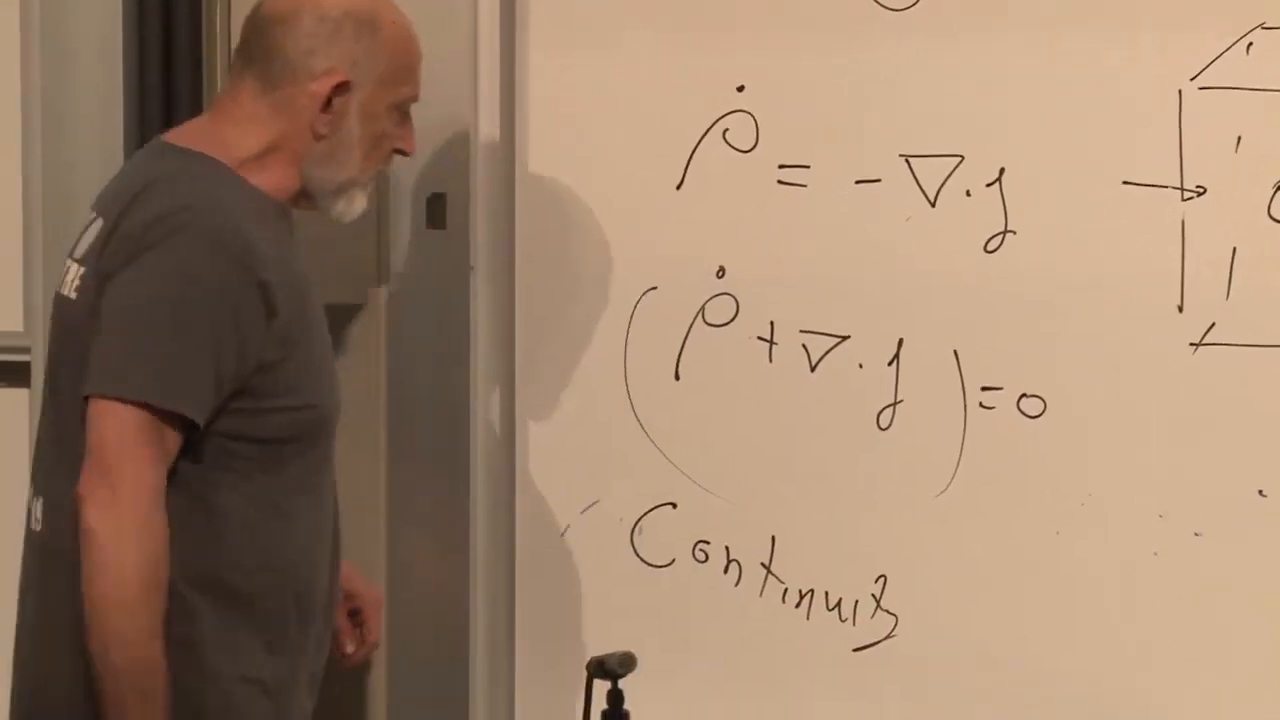
\includegraphics[width=\linewidth]{lecture_08_figure_16.png}
\caption{局所的な釣り合いの法則
\(\dot\rho=-\boldsymbol\nabla\cdot\mathbf J\)と、その境界電流がそれを生み出す小さな箱。}
\par\smallskip
\textit{講義フレーム：01：20：45。}
\end{figure}

これは慣習的に連続の方程式と呼ばれる。講義では\emph{局所保存}という名称を好む。連続性という言葉は数学的な滑らかさの仮定を連想させうるが、物理的内容は、電荷がここで消えてそこに現れるには、その間に電流がなければならないということである。

\subsection{なぜマクスウェルは変位電流を必要としたか}

式~\eqref{eq:continuity}はマクスウェル方程式への独立な追加ではない。ガウスの法則の時間微分と、アンペール--マクスウェルの法則の発散を取ると、
\begin{align}
\frac{\partial\rho}{\partial t}
&=
\boldsymbol\nabla\cdot
\frac{\partial\mathbf E}{\partial t},
\\
-\boldsymbol\nabla\cdot\mathbf J
&=
\boldsymbol\nabla\cdot
(\boldsymbol\nabla\times\mathbf B)
+
\boldsymbol\nabla\cdot
\frac{\partial\mathbf E}{\partial t}
\\
&=
\boldsymbol\nabla\cdot
\frac{\partial\mathbf E}{\partial t}.
\end{align}
したがって二つの左辺は等しく、
\(\partial_t\rho=-\boldsymbol\nabla\cdot\mathbf J\)、すなわちちょうど式~\eqref{eq:continuity}が得られる。構造上重要なのは、\(\mathbf E\)の時間微分、すなわち変位電流の項が、発散の関係が電荷保存と両立するために不可欠であるということである。

\begin{classroomqa}
\audiencequestion{我々は、二つの源をもつマクスウェル方程式がどこから来るのかを示していませんね？}
\lecturerresponse{いいえ。それらは力学の目標であり、次回作用から導かれる。静磁場の回転の法則はマクスウェル以前から知られていた。マクスウェルの決定的な時間依存の追加は変位電流であった。その存在により、場の方程式は局所的な電荷保存と両立する。\lecturetimestamp{01:23:15}}
\end{classroomqa}

詳細な発散の計算は講義では演習として残されるが、その結論は任意ではない。マクスウェル方程式は電荷保存を要求する。

\section{四元電流とその発散}

式~\eqref{eq:continuity}を成分で書くと、
\begin{equation}
\frac{\partial\rho}{\partial t}
+
\frac{\partial J_x}{\partial x}
+
\frac{\partial J_y}{\partial y}
+
\frac{\partial J_z}{\partial z}
=0.
\label{eq:continuity-components}
\end{equation}

\begin{figure}[H]
\centering
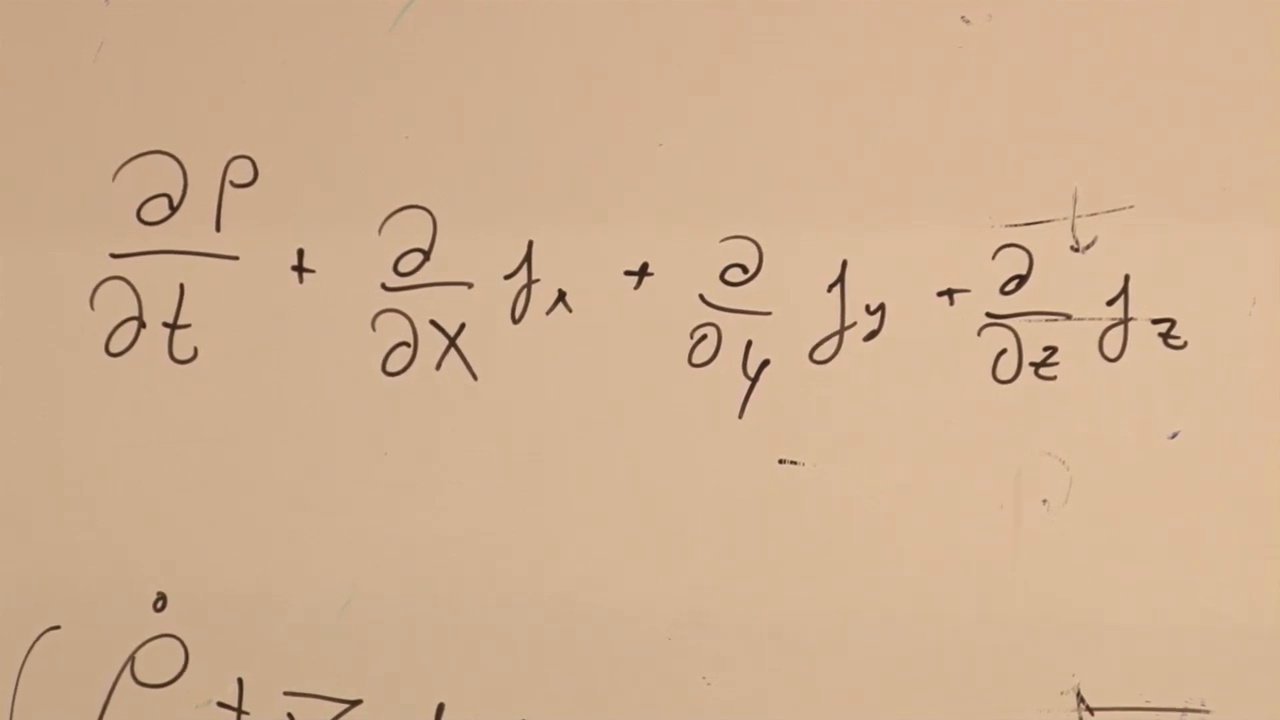
\includegraphics[width=\linewidth]{lecture_08_figure_17.png}
\caption{局所的な電荷保存を、一つの時間微分と三つの空間微分に展開したもの。}
\par\smallskip
\textit{講義フレーム：01：25：40。}
\end{figure}

\(J^\mu\)が式~\eqref{eq:four-current}で定義されると、四つの項は一つの縮約である：
\begin{equation}
\boxed{\partial_\mu J^\mu=0}.
\label{eq:four-current-conservation}
\end{equation}
\(\partial_\mu\)の下付き添字は\(J^\mu\)の上付き添字と縮約するので、結果はローレンツスカラーである。幾何学的な窓の構成はすでにこの変換則を示唆していた。\(\rho\)と三つの電流成分は、同じ電荷流束の四つの向きである。

\begin{figure}[H]
\centering
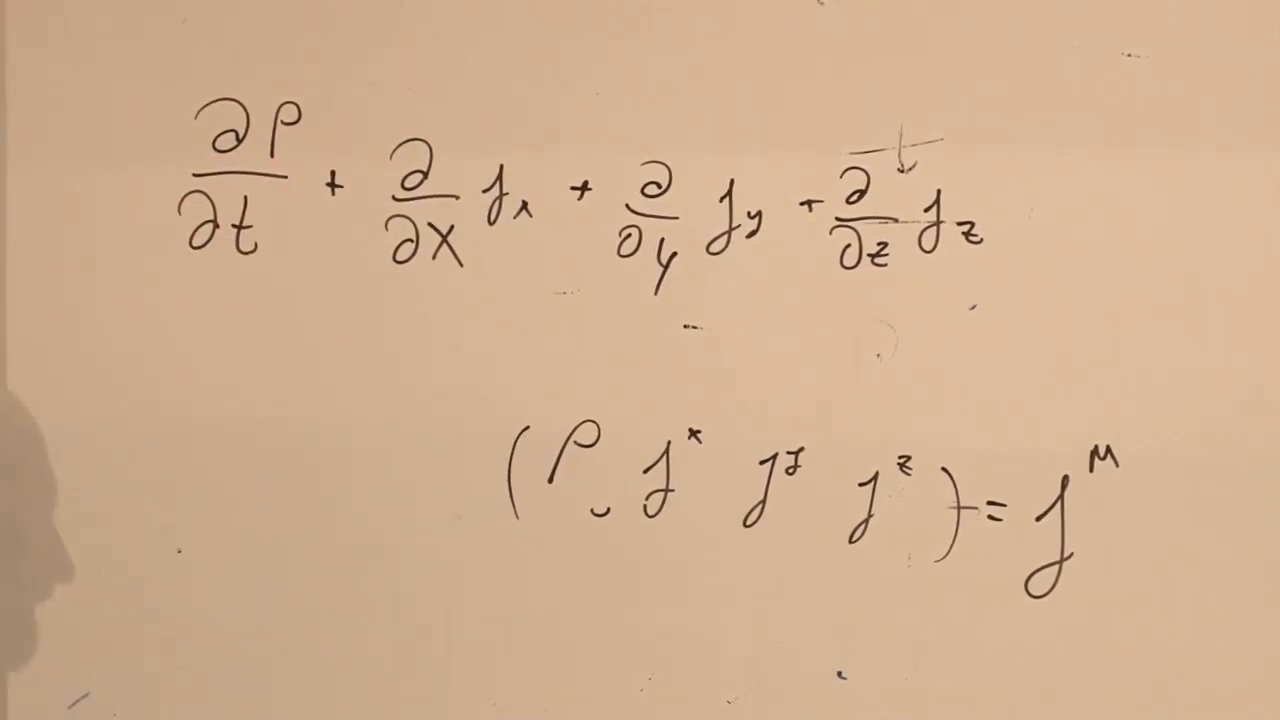
\includegraphics[width=\linewidth]{lecture_08_figure_18.png}
\caption{成分\((\rho,J_x,J_y,J_z)\)を\(J^\mu\)にまとめ、四元勾配と縮約したもの。}
\par\smallskip
\textit{講義フレーム：01：27：10。}
\end{figure}

\begin{classroomqa}
\audiencequestion{いつ\(\rho\)の時間微分が偏微分になったのですか？}
\lecturerresponse{最初から偏微分でした。空間的な箱を固定し、時間が変化するにつれてその電荷密度がどのように変化するかを問うています。動く軌道を追っているのではないので、ここでの\(\dot\rho\)は\(x,y,z\)を固定した\(\partial\rho/\partial t\)を意味します。\lecturetimestamp{01:28:20}}
\end{classroomqa}

\section{共変形式での同次方程式}

これで必要な対象が揃った：
\begin{itemize}
\item \(\mathbf E\)と\(\mathbf B\)は反対称テンソル\(F_{\mu\nu}\)の六つの独立成分であり、
\item \(\rho\)と\(\mathbf J\)は\(J^\mu\)の四つの成分であり、
\item 局所保存はスカラー方程式
\(\partial_\mu J^\mu=0\)である。
\end{itemize}
この講義の残りの課題は、同次マクスウェル方程式の対、式~\eqref{eq:homogeneous-div}と
\eqref{eq:homogeneous-curl}を、一つのテンソル方程式として書くことである。

\subsection{巡回微分}

答えは
\begin{equation}
\boxed{
\partial_\sigma F_{\nu\tau}
+
\partial_\nu F_{\tau\sigma}
+
\partial_\tau F_{\sigma\nu}
=0
}.
\label{eq:bianchi}
\end{equation}
三つの項は、微分の添字と二つの場のテンソルの添字を巡回的に割り当てる。これはしばしば
\begin{equation}
\partial_{[\sigma}F_{\nu\tau]}=0,
\end{equation}
と略記される。ここで括弧は反対称化を表す。

\begin{figure}[H]
\centering
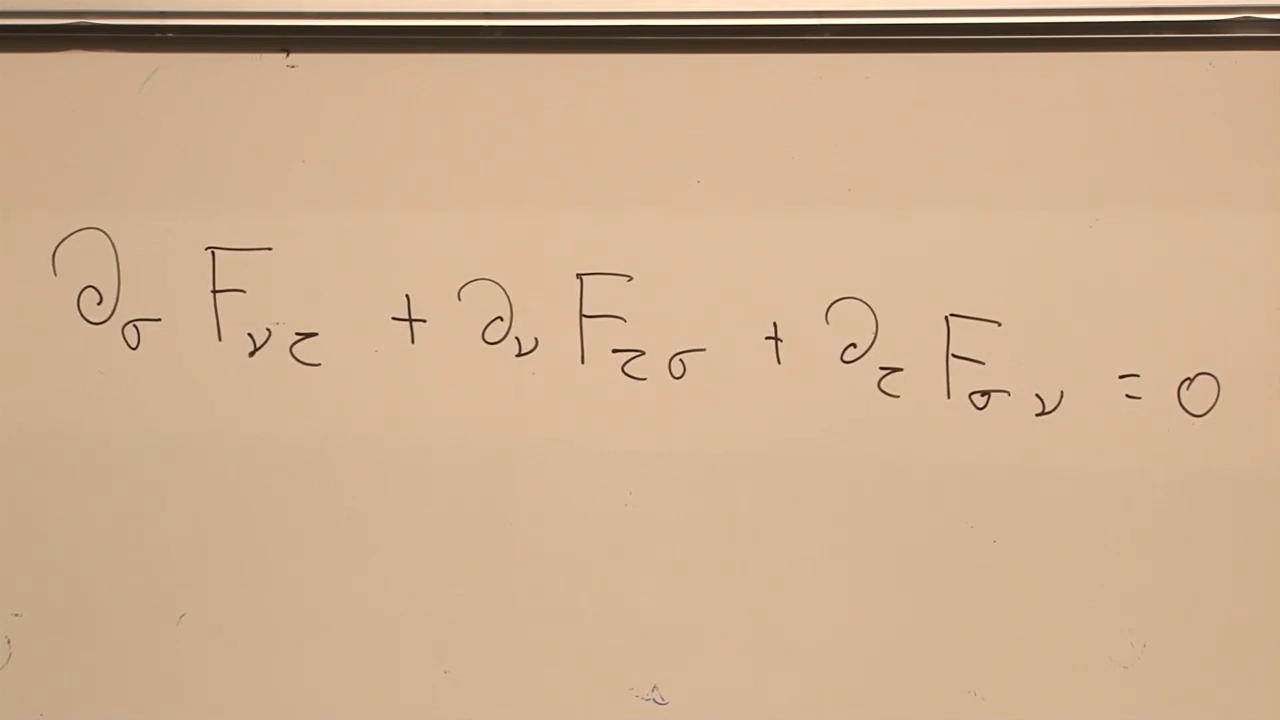
\includegraphics[width=\linewidth]{lecture_08_figure_19.png}
\caption{同次マクスウェル方程式をまとめる巡回三添字方程式。}
\par\smallskip
\textit{講義フレーム：01：33：20。}
\end{figure}

\subsection{三つの添字がすべて空間的}


\begin{equation}
(\sigma,\nu,\tau)=(x,y,z).
\end{equation}
と置くと、
\begin{align}
0
&=
\partial_xF_{yz}
+
\partial_yF_{zx}
+
\partial_zF_{xy}
\\
&=
\partial_xB_x+\partial_yB_y+\partial_zB_z
\\
&=
\boldsymbol\nabla\cdot\mathbf B.
\end{align}
したがって式~\eqref{eq:bianchi}の全空間成分は、まさに磁場の発散の不在である。

\begin{figure}[H]
\centering
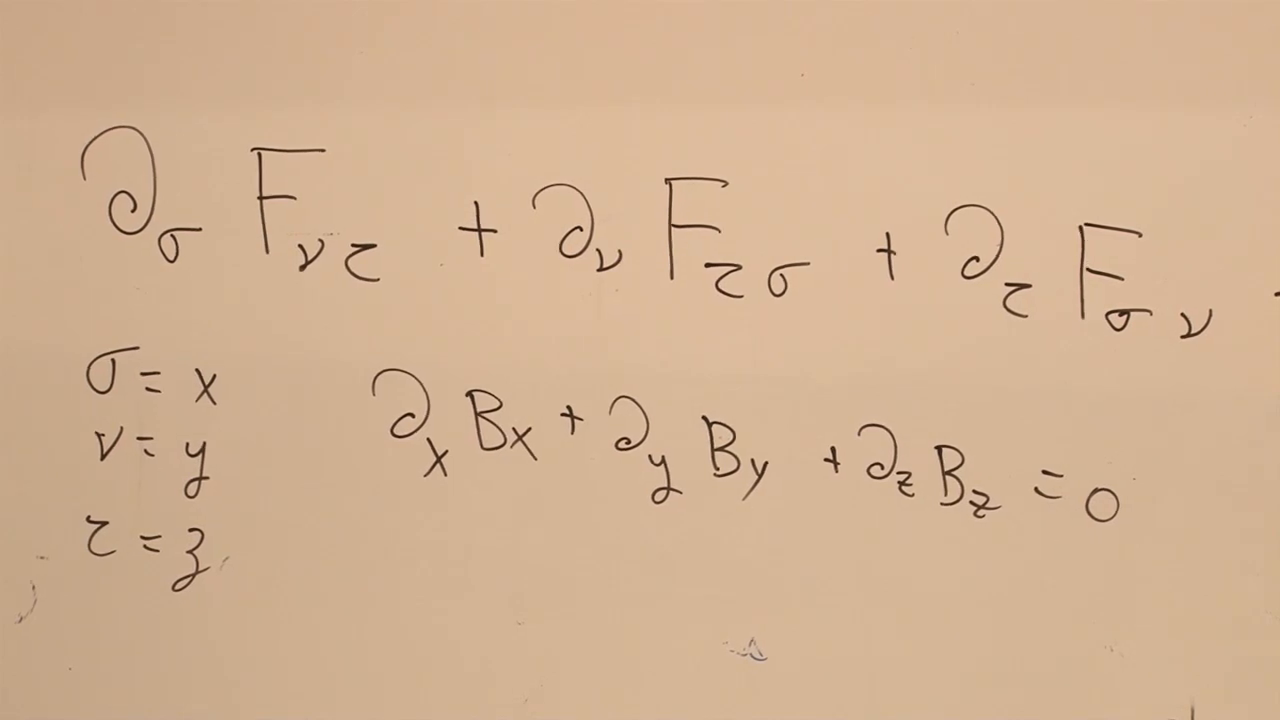
\includegraphics[width=\linewidth]{lecture_08_figure_20.png}
\caption{巡回恒等式の全空間成分は\(\partial_xB_x+\partial_yB_y+\partial_zB_z=0\)に帰着する。}
\par\smallskip
\textit{講義フレーム：01：35：30。}
\end{figure}

\subsection{一つの時間添字}

例えば、
\begin{equation}
(\sigma,\nu,\tau)=(y,x,0).
\end{equation}
と選ぶ。すると式~\eqref{eq:bianchi}は、電場成分の二つの空間微分と磁場成分の一つの時間微分を組み合わせる：
\begin{equation}
\partial_yF_{x0}
+
\partial_xF_{0y}
+
\partial_0F_{yx}
=0.
\end{equation}
式~\eqref{eq:f-lower-matrix}の行列を用いると、これは
\begin{equation}
\boldsymbol\nabla\times\mathbf E
-\frac{\partial\mathbf B}{\partial t}
=\mathbf0,
\end{equation}
の一つの成分であり、相対的な符号は反対称性によって固定される。他の空間添字の対を選ぶと、残りの二つの回転成分が得られる。

\begin{figure}[H]
\centering
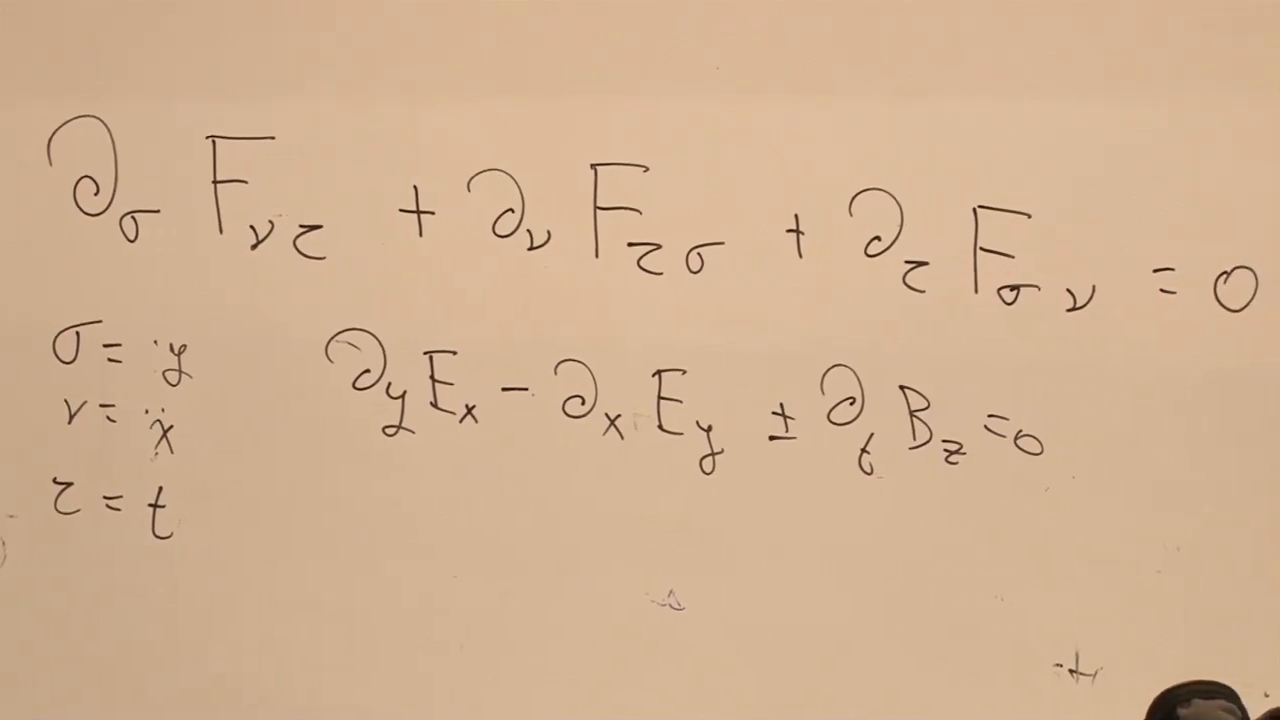
\includegraphics[width=\linewidth]{lecture_08_figure_21.png}
\caption{ファラデーの方程式の1つの成分を導出する、一度限りの2つの空間成分の検査。}
\par\smallskip
\textit{講義フレーム：01:38:20。}
\end{figure}

直接的な証明もある。式~\eqref{eq:field-tensor-definition}を式~\eqref{eq:bianchi}に代入する。6つの二階導関数の項が現れ、偏導関数が可換であるため、対になって相殺する。これは、回転の発散および勾配の回転の恒等式の四次元版である。

\begin{classroomqa}
\audiencequestion{ビアンキという名前に\(h\)はあるか。}
\lecturerresponse{はい。巡回方程式は電磁ビアンキ恒等式であり、一般相対性理論にも現れる幾何学的恒等式の特別な場合である。そのより深い幾何学的解釈は後回しにする。
\lecturetimestamp{01:40:28}}
\end{classroomqa}

\subsection{なぜ64個の書かれた成分が4つの方程式しか含まないのか}

3つの添字がそれぞれ4つの可能な値を持つため、\(4^3=64\)個の方程式が生じるように見える。反対称性が冗長性を取り除く：
\begin{itemize}
\item 任意の2つの添字が一致する場合、巡回表現は恒等的に消える。
\item 3つの添字がすべて異なる場合、置換は符号を除いて同じ方程式を再現する。
\item 四次元には、異なる添字の順序なし三つ組が\(\binom{4}{3}=4\)個しかない。
\end{itemize}
すべての添字が異なる順序付き三つ組は\(24\)個あり、6つの置換からなる4つの組にまとめられる。残りの\(40\)個の順序付き三つ組は消える。4つの独立な方程式は、1つの磁場の発散方程式とファラデーの方程式の3つの成分である。

\begin{classroomqa}
\audiencequestion{場のテンソルは6つの独立な成分を持つが、3添字の表現は64個の方程式を含むように見える。なぜ4つだけが残るのか。}
\lecturerresponse{繰り返された添字はゼロを与え、3つの異なる添字の置換は符号を除いて同じ関係を繰り返す。したがって、見かけ上64個の成分は4つの独立な方程式に縮約される。
\lecturetimestamp{01:41:58}}
\end{classroomqa}

式~\eqref{eq:bianchi}は明らかにテンソル的であり、したがってローレンツ共変である。滑らかな単一ポテンシャル記述では、磁荷密度も磁流も存在しないことも述べている。動的な源を持つ対は、講義で到達したまさにその境界に残される：その共変方程式と作用の導出は次回に属する。

\section{双対性とモノポールの問題}

最後の問いは、電気的源と磁気的源の間の見かけの非対称性に戻る。空空間では、マクスウェル方程式は電気--磁気双対回転
\begin{equation}
\mathbf E\longrightarrow\mathbf B,
\qquad
\mathbf B\longrightarrow-\mathbf E.
\label{eq:duality-quarter-turn}
\end{equation}
を持つ。これは軸\(\mathbf E\)と\(\mathbf B\)を持つ抽象的な平面内での90度の回転であり、単にそれらのラベルを交換する反射ではない。電気的源と磁気的源の両方が存在する場合、電気的四元電流と磁気的四元電流は同時に回転しなければならない。

\begin{figure}[H]
\centering
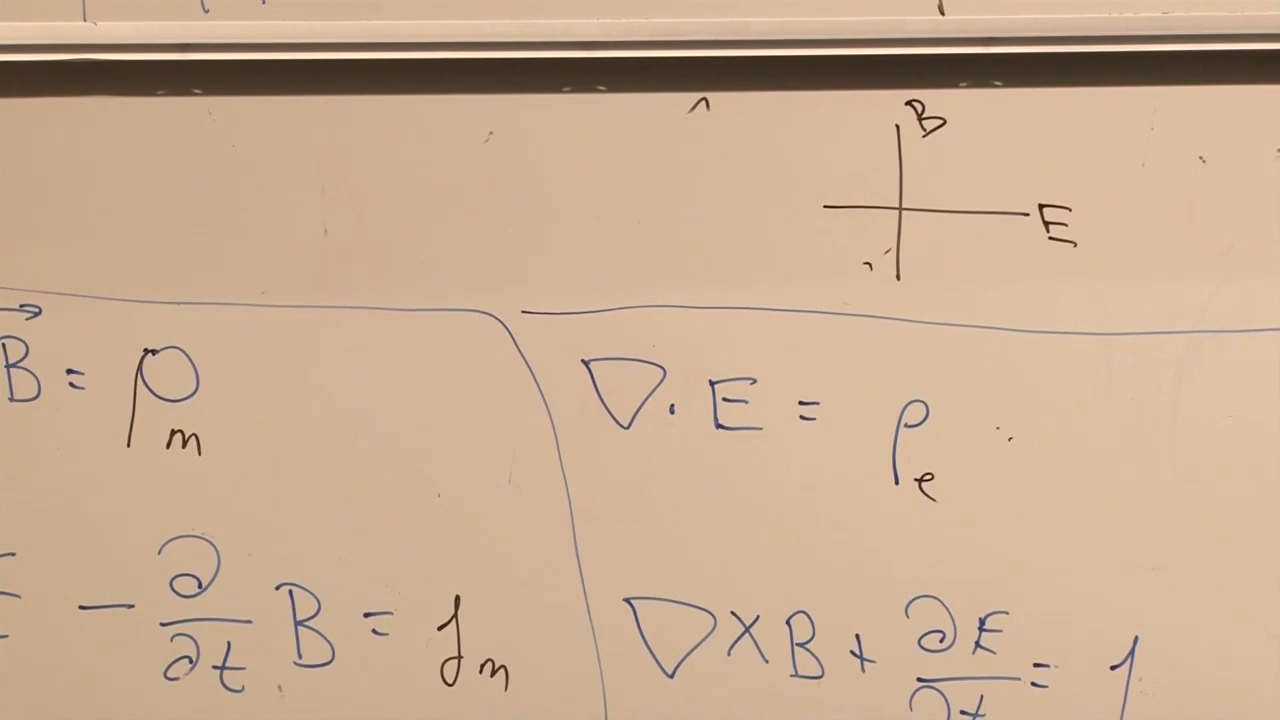
\includegraphics[width=\linewidth]{lecture_08_figure_22.png}
\caption{結びの電気--磁気双対図：単純な交換ではなく、\(E\)-\(B\)平面内での4分の1回転。}
\par\smallskip
\textit{講義フレーム：01:45:00。}
\end{figure}

\begin{classroomqa}
\audiencequestion{源のない方程式が電気と磁気の交換の下で双対であるなら、なぜ電気的成分は時間--空間成分であり、磁気的成分は空間--空間成分なのか。}
\lecturerresponse{その区別は\(F_{\mu\nu}\)内でフレーム依存的であり、源のない方程式は双対回転を許す。正しい操作は
\(\mathbf E\to\mathbf B\)および
\(\mathbf B\to-\mathbf E\)であり、磁荷が含まれる場合は源電流も同様に回転する。直接的な交換では必要な符号を見落とす。\lecturetimestamp{01:43:25}}
\end{classroomqa}

\begin{classroomqa}
\audiencequestion{清潔なテンソル描像は磁気モノポールを無意味にするのか。}
\lecturerresponse{いいえ。それは、モノポールが空間全体にわたって1つの滑らかなベクトルポテンシャルで表現できないことを意味する。代わりに、ポテンシャルはパッチを当てるか、ゲージ依存的に特異にするか、等価な双対記述に置き換えなければならない。素電荷の磁気モノポールは観測されておらず、講義は夜の終わりに問題を押し付けるのではなく、モノポールが形式主義にどのように適合するかに戻ると約束する。
\lecturetimestamp{01:45:50}}
\end{classroomqa}

したがって、講義は正確なフロンティアで終わる。相対性理論は、なぜ電場と磁場が混ざるのかを説明した。ポテンシャルの定義は、均質なマクスウェル方程式とそのビアンキ形式を与えた。電荷の流れは四元電流となり、局所保存は\(\partial_\mu J^\mu=0\)となった。残るのは動的なものである：電磁作用と共変な源を持つ場の方程式。